
\documentclass[twocolumn]{revtex4}


\usepackage[]{graphicx}

\begin{document}


\title{
CSIS Final
}

\author{J.~Doran}
\affiliation{Siena College, Loudonville, NY}

\date{\today}

\begin{abstract}
 	This document will explain and analyze the outcome of whether or not you can outrun a raptor or not. For this experiment, we were given a initial velocity of 18m/s for the raptor, and an initial velocity of 3m/s for you, both you and a raptor have a acceleration of 0, and only you have an initial distance of 30m. With this given information, we were able to calculate the time it would take for the raptor to catch up to you, the time it would take for the raptor to be at the right distance to take its first bite(1m), and the probability of all three bites to see if it actually bites you. 
 	 
\end{abstract}

\maketitle

\section{Explanation}
	The first step in this experiment was to create a line graph of both you and the raptor's position vs. time.  I did this by importing the matlab and numpy functions that are stored into python. I made the equations for both of the lines by using the formula {\it $y=mx+b$}. Since it's a position vs. time graph, the velocity is the slope and y-intercept is the initial distance so we get for the raptor {\it $y=18x$} and for you we get {\it $y=3x+30$}. Then I implemented a for loop to calculate all of the points that follow the equations. 
	To calculate the time that you and the raptor meet, we used another for loop. We set both of the equations equal to variables and then set them equal to a boolean to return the value of the time at which they two equations are equal. 
	To calculate the time when the raptor is a meter behind you, we used the same for loop but instead changing the raptor equation to {\it $y=18x+1$}.  And for the plot we used the same code for the first plot but we added in {\it $plt.arrow(1.94,21,0.0,10,head_width=.1,head_length=3)$ } to create an arrow pointing at the point of where the raptor is 1m behind. 
	
\section{Equations}
I used the formula $y=mx+b$ to make the equations for the lines. The slope would be velocity and the y-intercept would be the intial distance of either the raptor or you. 
$$y=3x+30$$
$$y=18x$$

To solve for how long it took the raptor to catch up to you I set the distance formula of the raptor equal to the distance of you:
$$ x_0 + v_ot +\frac{1}{2}at^2=x_0 + v_ot +\frac{1}{2}at^2$$


To find the probability of the raptor biting during the chase i used:
$$chase probability= (amount of escapes/number of tries) *100$$




\section{Graphs}
\begin{figure} 
   
    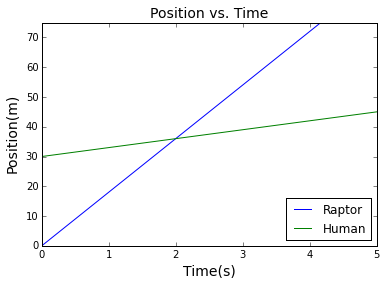
\includegraphics[width=0.5\textwidth]{PvsT1.png}
    \caption{This is the position vs. time graph when you and the raptor meet.\label{fig:graph}}
\end{figure}
\begin{figure} 
   
    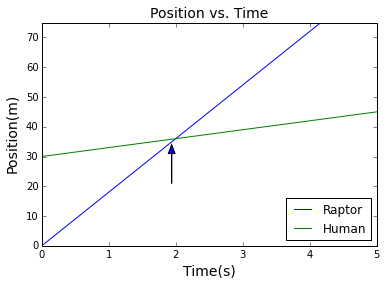
\includegraphics[width=0.5\textwidth]{PvsT2.png}
    \caption{This is the position vs. time graph when the raptor is a meter behind you.\label{fig:graph}}
\end{figure}




\end{document}
